% Created 2017-02-06 Mon 00:55
% Intended LaTeX compiler: pdflatex
\documentclass[11pt]{article}
\usepackage[utf8]{inputenc}
\usepackage[T1]{fontenc}
\usepackage{graphicx}
\usepackage{grffile}
\usepackage{longtable}
\usepackage{wrapfig}
\usepackage{rotating}
\usepackage[normalem]{ulem}
\usepackage{amsmath}
\usepackage{textcomp}
\usepackage{amssymb}
\usepackage{capt-of}
\usepackage{hyperref}
\author{Bhupendra}
\date{\today}
\title{Intro to Algorithms: CLRS}
\hypersetup{
 pdfauthor={Bhupendra},
 pdftitle={Intro to Algorithms: CLRS},
 pdfkeywords={},
 pdfsubject={},
 pdfcreator={Emacs 24.5.1 (Org mode 9.0.1)}, 
 pdflang={English}}
\begin{document}

\maketitle
\tableofcontents


\section{Part1: Foundations}
\label{sec:orgee23445}

\subsection{Chapter2: Getting Started}
\label{sec:orgb370f73}
\subsubsection{Merge Sort}
\label{sec:orge60101e}

\begin{enumerate}
\item Algorithm
\label{sec:orgcc5e894}
\begin{verbatim}
# To sort A call MergeSort(A,0,len(A)-1)
def MergeSort(A,p,r):
    if p<r:
        q=(p+r)/2
        MergeSort(A,p,q)
        MergeSort(A,q+1,r)
        Merge(A,p,q,r)
\end{verbatim}

\begin{verbatim}
# function to merge A[p:q] and A[q+1:r]
def Merge(A,p,q,r):
    n1 = q-p+1
    n2 = r-q
    L = [None]*(n1+1)
    R = [None]*(n2+1)
    for i in range(0,n1,1):
        L[i]=A[p+i]
    for j in range(0,n2,1):
        R[j]=A[q+j+1]
    L[n1] = float("inf")
    R[n2] = float("inf")
    i=0
    j=0
    for k in range(p,r+1,1):
        if L[i] <= R[j]:
            A[k]=L[i]
            i=i+1
        else:
            A[k]=R[j]
            j=j+1
\end{verbatim}

\item Correctness
\label{sec:org1523936}
Defining the following loop invariant: \\
At the start of each iteration of the for loop of lines 22-28,
\begin{enumerate}
\item the subarray \(A[p..k-1]\) contains the \(k-p\) smallest elements of \(L[0..n1]\) and \(R[0..n2]\), in sorted order.
\item Moreover, \(L[i]\) and \(R[j]\) are the smallest elements of their arrays that have not been copied back into \(A\). \\
\end{enumerate}

\textbf{Initialization:} 1) \(k=p\),  A[p..k-1] is empty: k-p=0 smallest elements.
2)\(i=j=1\), L[1] and R[1] are the smallest elements that have not copied back to A. \\

\textbf{Induction:} Suppose L[i]\(\le\) R[j], then L[i] is the smallest element not yet copied back in A and line 24 do that. 
As subarray A[p..k-1] contained the k-p smallest element initially now it has k-p+1 smallest elements and then k is incremented
to hold the 1st point of loop invariant. i is also incremented which maintain 2nd point of loop invariant. Similarly is L[i]>R[i]
appropriate actions are taken to maintain the loop invariant. \\

\textbf{Termination:} k=r+1, at this point A[p..r] is sorted and contain r+1-p smallest element of L and R which are of A. So now 
we have sorted array A.

\item Analyzing Merge Sort
\label{sec:org1777c67}
There are three steps:
\begin{enumerate}
\item Divide: O(1)
\item Conquer: \(2T(n/2)\), solving two sub-problems of n/2 sizes.
\item Combine: O(n), In Merge for loop from lines 22 to 28 runs n times.
\end{enumerate}
which gives \\
\begin{equation}
T(n) = \begin{cases}
\theta(1), & \text{if $n=1$}.\\
2T(n/2) + \theta(n), & \text{if $n>1$}.
\end{cases}
\end{equation}

using recursion tree \begin{center}
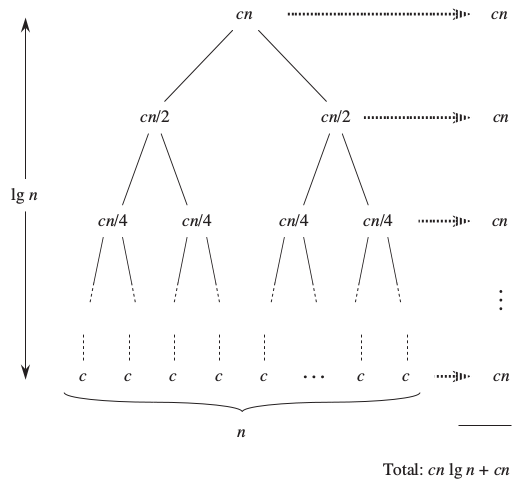
\includegraphics[width=.9\linewidth]{./img/mergesort.png}
\end{center}

thus T(n) = O(n \(\log\) n).
\end{enumerate}
\subsection{Chapter4: Divide and Conquer}
\label{sec:org171b1db}
\subsubsection{Maximum Subarray Problem}
\label{sec:org316d8c3}
\begin{verbatim}
def Find_Max_Crossing_Subarray(A,low,mid,high):
    left_sum=-float("inf")
    sum=0
    for i in range(mid,low-1,-1):
        sum=sum+A[i]
        if sum>left_sum:
            left_sum=sum
            max_left=i
    right_sum=-float("inf")
    sum=0
    for j in range(mid+1,high+1,1):
        sum=sum+A[j]
        if sum>right_sum:
            right_sum=sum
            max_right=j
    return(max_left,max_right,left_sum+right_sum)
\end{verbatim}

\begin{verbatim}
def Find_Max_Subarray(A,low,high):
    if high==low:
        return (low,high,A[low]) # base case
    else:
        mid = (low+high)/2
        (left_low,left_high,left_sum)=Find_Max_Subarray(A,low,mid)
        (right_low,right_high,right_sum)=Find_Max_Subarray(A,mid+1,high)
        (cross_low,cross_high,cross_sum)=Find_Max_Crossing_Subarray(A,low,mid,high)

        if left_sum>=right_sum and left_sum>=cross_sum:
            return (left_low,left_high,left_sum)
        elif right_sum>=left_sum and right_sum>=cross_sum:
            return (right_low,right_high,right_sum)
        else:
            return (cross_low,cross_high,cross_sum)
\end{verbatim}

Analyzing the divide and conquer algorithm:

\begin{equation}
T(n) = \begin{cases}
\theta(1), & \text{if $n=1$}.\\
2T(n/2) + \theta(n), & \text{if $n>1$}.
\end{cases}
\end{equation}

\subsubsection{Substitution method for solving recurrences}
\label{sec:org6984e1c}
\begin{enumerate}
\item Guess the form of the solution
\item Verify: Show the solution works
\item Find constants mathematical induction
\end{enumerate}
we substitute the guessed solution for the problem when applying the inductive hypothesis to smaller values; hence the name substitution method.

For solving the above equation we guess that the solution is \(T(n)=\theta(n \log n)\).Assume this solution holds for all \(m < n\) , in particular for \(m = n/2\) , yielding
T(n/2) \(\le\) \(c n/2 \log n/2\). Substituting in the recurrence equation gives

\begin{align*}
T(n) &\leq 2(c n/2 \log n/2) + n \\
&\leq c n \log n/2 + n \\
&= cn \log n - cn \log2 + n \\
&= cn \log n - cn + n \\
&\leq cn \log n & \forall c \geq 1
\end{align*}

\subsubsection{Recurrence tree method for solving recurrences}
\label{sec:orge7e9b86}

\subsubsection{Master method for solving recurrences}
\label{sec:orgdfcff68}
of the form
\begin{align*}
T(n) = aT(n/b) + f(n), & a\geq1 \& b>1
\end{align*}

\section{Part2: Sorting and Order Statistics}
\label{sec:orgbbd09bd}

\subsection{Chapter6: Heap Sort}
\label{sec:orgc07c923}
\(O (n \log n)\), in place

\subsubsection{Heap}
\label{sec:orgb640a25}
The heap data structure is an array object that we can view as a near complete binary tree.
Each node of the tree corresponds to an element in the array. Root of the tree is A[1] and
\begin{verbatim}
def Parent(i):
    return i/2
def Left(i):
    return 2*i
def Right(i):
    return 2*i+1
\end{verbatim}
\textbf{max-heap} : A[Parent(i)] \(\ge\) A[i] \\
\textbf{min-heap} : A[Parent(i)] \(\le\) A[i]
\subsubsection{Algorithm}
\label{sec:org94f0912}
\textbf{Max-Heapify} : in worst case when bottom level is half filled
\begin{equation}
T(n) <= T(2n/3) + \theta (1)
\end{equation}
whose solution by master theorem case 2 is \$ O( \(\log\) n) \$
\begin{verbatim}
# maintain heap property for one violation at i
def Max_Heapify(A,i,heap_size=None):
    if heap_size == None:
        heap_size = len(A)
    l=Left(i)
    r=Right(i)
    if l<=heap_size and A[l]>A[i]:
        largest = l
    else:
        largest = i
    if r<=heap_size and A[r]>A[largest]:
        largest = r
    if largest != i:
        A[i],A[largest] = A[largest], A[i]
        Max_Heapify(A,largest)
\end{verbatim}

\textbf{Build-Max-Heap} : 
$$ \sum_{c=0}^{\log n} c*n/2^c+1 = c*n / 2 $$
\implies \$ O(n) \$
\begin{verbatim}
def Build_Max_Heap(A):
    for i in range(len(A)/2,1,-1):
        Max_Heapify(A,i)
\end{verbatim}

\textbf{Heap-Sort} :
\begin{verbatim}
def HeapSort(A):
    Build_Max_Heap(A)
    heap_size = len(A)
    for i in range(len(A),1,-1):
        index=i-1
        A[1],A[index] = A[index],A[1]
        heap_size -=1
        Max_Heapify(A,index,heap_size)
\end{verbatim}

\subsection{Chapter7: Quick Sort}
\label{sec:org92a7881}
\subsubsection{Algorithm}
\label{sec:org0d309ac}
\begin{verbatim}
1  # To sort A call (A,0,len(A)-1)
2  def QuickSort(A,p,r):
3      if p<r:
4          q=Partion(A,p,r)
5          QuickSort(A,p,q-1)
6          QuickSort(A,q+1,r)
\end{verbatim}

\begin{verbatim}
 7  # function to partion A and place pivot at an appropriate position
 8  def Partion(A,p,r):
 9      x=A[r]
10      i=p-1
11      for j in range(p,r):
12          if A[j]<=x:
13              i=i+1
14              A[i],A[j]=A[j],A[i]
15      A[i+1],A[r] = A[r],A[i+1]
16      return i+1
\end{verbatim}

\subsubsection{Correctness}
\label{sec:orgd682bef}
loop invariant for line 11-15, let k be an index 0 \(\le\) k \(\le\) n then
\begin{enumerate}
\item if p \(\le\) k \(\le\) i then A[k] \(\le\) x
\item if i+1 \(\le\) k \(\le\) j-1 then A[k] > x
\item if k=r then A[k] = x \\
\end{enumerate}

\textbf{Initialization:} initially i=p-1 and j=p then 1) no values between p and i implies A[k] \(\le\) x, similarly between i+1 and j-1 
no values implies A[k]>x , Also \(A[r]=x\).

\textbf{Induction:} \begin{center}
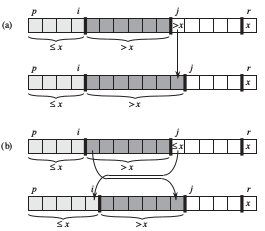
\includegraphics[width=.9\linewidth]{./img/quicksort_correctness.png}
\end{center}
a) Figure (a) shows what happens when A[j] > x;the only action in the loop is to increment j . After j is incremented, condition 2
holds for A[j-1] and all other entries remain unchanged.\\
b) Figure (b) shows what happens when A[j] \(\le\) x; the loop increments i, swaps A[i] and A[j], and then increments j . 
Because of the swap, we now have that A[i] \(\le\) x, and condition 1 is satisfied. Similarly, we also have that A[j]> x, since the
item that was swapped into A[j-1]is, by the loop invariant, greater than x.

\textbf{Termination:} when j=r and at that point. 1) A[p\ldots{}i] \(\le\) x. 2) \(A[i+1...r-1]>x\). 3) A[r]=x.At last we exchange pivot with 
leftmost element greater then x and move it to its correct position.

\subsubsection{Analyzing Quick Sort}
\label{sec:org10c0b3e}
Running time of Partition(A,p,r) = \(\theta\) (n) as for loop runs for n=r-p+1 times. \\
1 Worst case partitioning : Sub-problems have 0 and (n-1) size.
\begin{align*}
T(n) = T(n-1) + \theta(n)
\end{align*}
whose solution is
\begin{equation}
T(n) = \theta ( {n}^2 )
\end{equation}
\\
2 Best Case Partitioning: when both problems have size of n/2 then
\begin{align*}
T(n)=2T(n/2) + \theta (n)
\end{align*}
whose solution by master theorem is
\begin{equation}
T(n) = O (n \log n)
\end{equation}
\\
3 Average Case:
if there is some partitioning lets us say in 9/10 and 1/10 then
\begin{center}
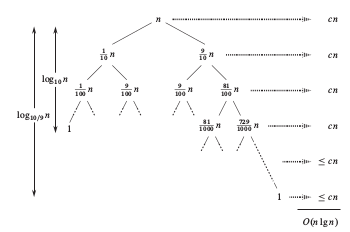
\includegraphics[width=.9\linewidth]{./img/quicksort_analyze.png}
\end{center}
which gives
\begin{equation}
T(n) = O (n \log n)
\end{equation}

\section{Part3: Data Structures}
\label{sec:org1cff466}

\subsection{Chapter12: Binary Search Tree}
\label{sec:org7024021}
A binary search tree is a binary tree such that for any node x, 
\begin{enumerate}
\item x.left.key <= x.key
\item x.right.key >=x
\end{enumerate}

\textbf{Sort} To print the keys in sorted order
\begin{verbatim}
def Inorder_Tree_Walk(root):
    if Root != None:
        Inorder_Tree_Walk(root.left)
        print root.key
        Inorder_Tree_Walk(root.right)
\end{verbatim}

\textbf{Search}
\begin{verbatim}
def Tree_Search(root,value):
    if root==None or value ==root.key:
        return root
    if value<root.key:
        return Tree_Search(root.left,value)
    else:
        return Tree_Search(root.right,value)
\end{verbatim}

\begin{verbatim}
def Iterative_Tree_Search(root,value):
    while root!=None and value!=root.key:
        if value<root.key:
            root=root.left
        else:
            root = root.right
    return root
\end{verbatim}
\end{document}